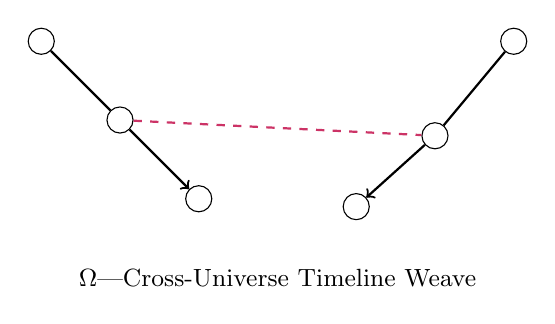
\begin{tikzpicture}[
    node/.style={circle,fill=white,draw=black,minimum size=5pt},
    arrow/.style={->, thick},
    contact/.style={draw=purple!80, thick, dashed}
]

% Universe A
\node[node] (A1) at (-3,1.0) {};
\node[node] (A2) at (-2,0.0) {};
\node[node] (A3) at (-1,-1.0) {};

\draw[arrow] (A1) -- (A2) -- (A3);

% Universe B
\node[node] (B1) at (3,1.0) {};
\node[node] (B2) at (2,-0.2) {};
\node[node] (B3) at (1,-1.1) {};

\draw[arrow] (B1) -- (B2) -- (B3);

% Contact edges
\draw[contact] (A2) -- (B2);

\node at (0,-2) {\small $\Omega$---Cross-Universe Timeline Weave};

\end{tikzpicture}